\section{Instant Messaging}

\frame{
  \frametitle{Inhaltsverzeichnis}
  \tableofcontents[currentsection]
}

\begin{frame}
  \frametitle{Open Source vs. Closed Source}
  \begin{definition}[Open Source]
   Programm mit öffentlich zugänglichem Quellcode \hfill \tiny [Duden]
  \end{definition}

  \begin{itemize}
   \item Programm kann von jedem geprüft werden
   \item Schwer Hintertüren einzubauen
   \item Notwenige Bedingung für prüfbar sichere Programme
   \item Open Source $\neq$ kostenlos
  \end{itemize}
\end{frame}

\begin{frame}
  \frametitle{Identitätsprüfung}
  \center
  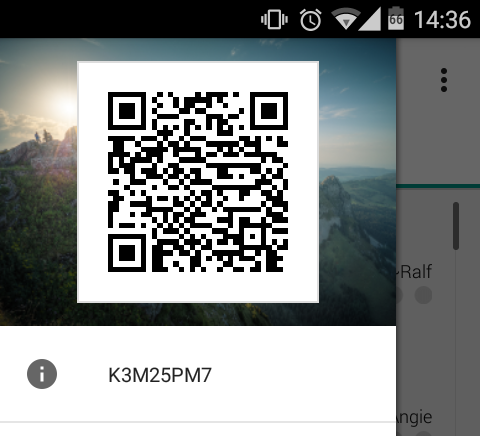
\includegraphics[width=0.6\textwidth]{figures/Threema_ID.png}
\end{frame}

\begin{frame}
  \frametitle{Perfect Forward Secrecy}
  Problem:
  \begin{itemize}
    \item Was passiert wenn der Schlüssel geklaut wird?
    \pause
    \item $\rightarrow$ Alle Nachrichten können entschlüsselt werden
    \item $\rightarrow$ Auch alte Nachrichten, die der Angreifer gespeichert hat
  \end{itemize}
  \pause
  Lösung:
  \begin{itemize}
    \item Sitzungsschlüssel (Analogie: Suppe)
  \end{itemize}
  \center \inputSVG[\def\svgscale{0.2}]{DH_soup}
\end{frame}

\begin{frame}
  \frametitle{Messaging App Scorecard der \textbf{E}lectronic \textbf{F}rontier \textbf{F}oundation (EFF)}
  \framesubtitle{Auszug aus \url{https://www.eff.org/secure-messaging-scorecard}}
  \center
  \tiny

  \newcommand{\myMarkSize}{0.5cm}
  \newcommand{\myCheck}{
\includegraphics[width=\myMarkSize]{eff_check}}
  \newcommand{\myCross}{
\includegraphics[width=\myMarkSize]{eff_cross}}
  \Wider[4.5em]{
  \begin{tabular}{@{} m{1.8cm}@{\hspace{1mm}} >{\centering\arraybackslash}m{1.7cm}@{\hspace{1mm}} >{\centering\arraybackslash}m{1.5cm}@{\hspace{1mm}} >{\centering\arraybackslash}m{1.2cm}@{\hspace{1mm}} >{\centering\arraybackslash}m{1.9cm}@{\hspace{1mm}} >{\centering\arraybackslash}m{1.0cm}@{\hspace{1mm}} >{\centering\arraybackslash}m{1.37cm}@{\hspace{1mm}} >{\centering\arraybackslash}m{0.6cm}@{\hspace{1mm}} @{}}
    \toprule \\
     & Transportweg\-verschlüs\-selung & Ende-zu-Ende verschlüsselt & Iden\-ti\-täts\-prü\-fung & Nachrichten sicher wenn Schlüssel geklaut & Open Source & Sicherheits\-konzept dokumentiert & Audit \\
    \midrule \\
    Facebook chat 	& \myCheck & \myCross & \myCross & \myCross & \myCross & \myCross & \myCheck \\
    Google Hangouts 	& \myCheck & \myCross & \myCross & \myCross & \myCross & \myCross & \myCheck \\
    iMessage 		& \myCheck & \myCheck & \myCross & \myCheck & \myCross & \myCheck & \myCheck \\
    Skype 		& \myCheck & \myCross & \myCross & \myCross & \myCross & \myCross & \myCross \\
    Whatsapp 		& \myCheck & \myCross & \myCross & \myCross & \myCross & \myCross & \myCheck \\
    Threema 		& \myCheck & \myCheck & \myCheck & \myCheck & \myCross & \myCheck & \myCross \\
    Textsecure		& \myCheck & \myCheck & \myCheck & \myCheck & \myCheck & \myCheck & \myCheck \\
    \bottomrule
  \end{tabular}}

\end{frame}
